% Prepared by Calvin Kent
%
% Assignment Template v19.02
%
%%% 20xx0x/MATHxxx/Crowdmark/Ax
%
\documentclass[12pt]{article} %
\usepackage{CKpreamble}
\usepackage{CKassignment}
\usepackage{tkz-euclide}
\usepackage{physunits}
\usepackage{physics}
\usepackage{mathtools}
\usepackage{lmodern}

\usepackage{pgfplots}
\usepgfplotslibrary{polar}
\usepgflibrary{shapes.geometric}
\usetikzlibrary{calc}


\usepackage{euscript}
\usepackage{microtype}
\usepackage{upgreek}
\usepackage[misc]{ifsym}


%%Title
\title{\textbf{Assignment 2 Functions - SOLUTIONS} \\ \textbf{Due Date: } Wednesday, January 19}
\date{January, 2022}

%%% Maths and science packages

\usepackage{amsmath,amsthm,amssymb}
\usepackage{pgfplots}
	\usetikzlibrary{
		calc,
		patterns,
		positioning
	}
	\pgfplotsset{
		compat=1.16,
		samples=200,
		clip=false,
		my axis style/.style={
			axis x line=middle,
			axis y line=middle,
			legend pos=outer north east,
			axis line style={
				->,
			},
			legend style={
				font=\footnotesize
			},
			label style={
				font=\footnotesize
			},
			tick label style={
				font=\footnotesize
			},
			xlabel style={
				at={
					(ticklabel* cs:1)
				},
				anchor=west,
				font=\footnotesize,
			},
			ylabel style={
				at={
					(ticklabel* cs:1)
				},
				anchor=west,
				font=\footnotesize,
			},
			xlabel= $x$,
			ylabel=$\vec d (\m \tx{[East]})$
		},
	}
	\tikzset{
		>=stealth
	}

\pgfplotsset{my style/.append style={axis x line=middle, axis y line=
middle, xlabel={$t$}, ylabel={$y[\text{m}]$}, axis equal }}

%%% Tables and figures packages

\usepackage{float}
\usepackage{caption}
	\captionsetup{
		format=plain,
		labelfont=bf,
		font=small,
		justification=centering
	}
	
%%% Numbers and sets

\newcommand{\E}{\mathrm{e}}

\newcommand{\tx}[1]{\text{#1}}
\newcommand{\rem}[1]{\operatorname{rem}{(#1)}}


%
\begin{document}
	\pagenumbering{arabic}
	% Start of class settings ...
	\renewcommand*{\coursecode}{MATH 235} % renew course code
	\renewcommand*{\assgnnumber}{Assignment 1} % renew assignment number
	\renewcommand*{\submdate}{September 14, 2021} % renew the date
	\renewcommand*{\studentfname}{Abdullah} % Student first name
	\renewcommand*{\studentlname}{Zubair} % Student last name
    \renewcommand*{\proofname}{Proof:}
	% \renewcommand*{\studentnum}{20836288} % Student number

	\renewcommand\qedsymbol{$\blacksquare$}
	\setfigpath
	% End of class settings	
	% \pagestyle{crowdmark}
	\newgeometry{left=18mm, right=18mm, top=22mm, bottom=22mm} % page is set to default values
	\fancyhfoffset[L,O]{0pt} % header orientation fixed
	% End of class settings
	%%% Note to user:
	% CTRL + F <CHANGE ME:> (without the angular brackets) in CKpreamble to specify graphics paths accordingly.
	% The command \circled[]{} accepts one optional and one mandatory argument.
	% Optional argument is for the size of the circle and mandatory argument is for its contents.
	% \circled{A} produces circled A, with size drawn for letter A. \circled[TT]{A} produces circled A with size drawn for TT.
	% https://github.com/CalvinKent/My-LaTeX
	%%%

	%%%%%%%%%%%%%%%%%%%%%%%%%%%%%%%%%%%%%%%%%%%%%%%%%%%%%%%%%%%%%%%%%%%%%%%%%%%%%%%
	%%%                        CUSTOM MACRO VIM-TEX                             %%%
	%%       call IMAP('NOM', '\nomenclature{}', 'tex')               

	%%%%%%%%%%%%%%%%%%%%%%%%%%%%%%%%%%%%%%%%%%%%%%%%%%%%%%%%%%%%%%%%%%%%%%%%%%%%%%%

	% Crowdmark assignment start
	% qnumber, qname, qpoints
\maketitle
	\section{Preamble}
  This assignment covers everything taught so far. The solutions that you hand in should be \textbf{neat} and \textbf{legible},
  this is an assignment, not a quiz, so I expect you to take your time and present thorough and detailed solutions.
\section{Name and Date:}
	Print your name and todays date below;\\


	\begin{center}
	\noindent\begin{tabular}{ll}
		\makebox[3in]{\hrulefill} & \makebox[3in]{\hrulefill}\\
		Name & Date\\[8ex]% adds space between the two sets of signatures
	\end{tabular}
	\end{center}
	\newpage



\begin{qstn}
  There exists a function that allows us to determine the length of a binary string.\\We call
  this function $\operatorname{len}$. Here a few examples to understand how it works,
  \begin{itemize}
    \item If $\textbf{S} = 1001$, then $\operatorname{len}(\textbf{S}) = 4$.
    \item If $\textbf{R} = 110001$, then $\operatorname{len}(\textbf{R}) = 6$.
    \item If $\textbf{T} = \epsilon$, then $\operatorname{len}(\textbf{T}) = 0$.
  \end{itemize}

  We can also define the operation of $ \textit{multiplication by a scalar}$ for binary strings. So suppose $n \in
  \mathbb N$ and \textbf{S} is some binary string, then,
    \[
      n\cdot \textbf{S} = \underbrace{\textbf{S} + \dots + \textbf{S}}_{\text{n times}}
    \]
  Again we resort to a few examples to demonstrate how multiplication by a scalar works,
  \begin{itemize}
    \item If $\textbf{S} = 1001$,  then $2\cdot\textbf{S} = \textbf{S} + \textbf{S} = 10011001$.
    \item If $\textbf{R} = 0$,  then $4\cdot\textbf{R} = \textbf{R} + \textbf{R} + \textbf{R} + \textbf{R} = 0000$.
    \item If $\textbf{T} = 01$,  then $3\cdot\textbf{T} = \textbf{T} + \textbf{T} + \textbf{T} = 010101$.
  \end{itemize}
  
Let $\textbf{S} = 001$ and $\textbf{T} = 11$, answer the following,
  \begin{enumerate}[label=(\alph*)]
    \item Let $\mathbb S$ represent the set of all binary strings. Define the length function using mapping
      notation. \vspace*{-0.5cm}
      \begin{solution}
        $\operatorname{len} \colon \mathbb S \rightarrow \mathbb N$.
      \end{solution}
    \item Compute $ \operatorname{len}(\textbf{S})$.
      \begin{solution}
         $ \operatorname{len}(\vb S) = \operatorname{len}(001) = 3$.
      \end{solution}
    \item Compute $ \operatorname{len}(\textbf{T})$.
      \begin{solution}
         $ \operatorname{len}(\vb T) = \operatorname{len}(11) = 2$.
      \end{solution}
    \item Compute $ \operatorname{len}(\textbf{S + T})$.
      \begin{solution}
        $ \operatorname{len}(\vb S + \vb T) = \operatorname{len}(001 + 11) = \operatorname{len}(00111) = 5$.
      \end{solution}
    \item Compute $ \operatorname{len}(3\cdot\textbf{S})$.
      \begin{solution}
      $ \operatorname{len}(3\cdot \vb S) = \operatorname{len}(3 \cdot 001) = \operatorname{len}(001001001) = 9$.
      \end{solution}
    \item Compute $ 3\cdot \operatorname{len}(\textbf{S})$.
      \begin{solution}
        $3 \cdot \operatorname{len}(\vb S) = 3 \cdot 3 = 9$.
      \end{solution}
    \item Compute $ \operatorname{len}(4\cdot\textbf{T})$.
      \begin{solution}
        $\operatorname{len}(4\cdot\textbf{T}) = \operatorname{len}(4 \cdot 11) = \operatorname{len}(11111111) = 8$.
      \end{solution}
    \item Compute $ 4\cdot \operatorname{len}(\textbf{T})$.
      \begin{solution}
        $4 \cdot  \operatorname{len}(\vb T) = 4 \cdot 2 = 8$.
      \end{solution}
  \end{enumerate}
\end{qstn}

\newpage

\begin{qstn}
  Let $F$ be a function. We call $F$ linear if both of the following conditions are satisfied,
  \begin{enumerate}
    \item For all inputs $x$ and $y$, 
      \[
          F(x+y) = F(x) + F(y)
      .\] 
    \item For all $c \in \mathbb F$, and all inputs $x$,
       \[
          F(c\cdot x) = c\cdot F(x)
      .\] 
  If $\mathbb F = \mathbb N$, then based on your results from Question 1, do you think that the length function, 
  $ \operatorname{len}$, is linear?
  Explain your answer.
  \end{enumerate}
  \begin{solution}
    From our results in parts (b),(c) we see that $ \operatorname{len}(\vb S) + \operatorname{len}(\vb T) = 3 +
    2 =  5$, and from  part (d) we see that $ \operatorname{len}(\vb S + \vb T) = 5$, hence it looks like the first
    condition of linearity is satisfied so far.

    From our result in part (e), we see that $\operatorname{len}(3\cdot \vb S) = 9$ and from part (f) we see 
    that  $3\cdot \operatorname{len}(\textbf{S}) = 9$, hence it looks like the second condition of linearity is
    satisfied as well.

    Combining our two hypothesis, we conclude that it appears like the length function is indeed linear.
  \end{solution}

\end{qstn}


\begin{qstn}
  Sometimes in math we would like a function that simply gets rid of trailing decimals and returns a whole number,
  aka an integer. This function is known as the floor function. We define it with mapping notation as $ \operatorname{floor} \colon
  \R \to \Z$, and it works as follows, if $x \in \R$, then $\operatorname{floor}(x)$ is the
  smallest integer that is less than or equal to $x$.
  Lets see how it works in the following examples,
  \begin{itemize}
    \item If $x = 4.2$, then $\operatorname{floor}(x) = \operatorname{floor}(4.2) =  4$.
    \item If $x = -7.4$, then $\operatorname{floor}(x) = \operatorname{floor}(-7.4) = -8$.
    \item If $x = 5$, then $\operatorname{floor}(x) = \operatorname{floor}(5) =  5$.
    \item If $x = 0.4$, then $\operatorname{floor}(x) = \operatorname{floor}(0.4) =  0$.
  \end{itemize}
\end{qstn}
\begin{enumerate}[label=(\alph*)]
  \item Compute $ \operatorname{floor}(2.5)$.
    \begin{solution}
      $ \operatorname{floor}(2.5) = 2$.
    \end{solution}
  \item Compute $ \operatorname{floor}(6 / 3)$.
    \begin{solution}
      $ \operatorname{floor}(6 / 3) = \operatorname{floor}(2) = 2$.
    \end{solution}
  \item Compute $ \operatorname{floor}(19 / 4)$.
    \begin{solution}
      $ \operatorname{floor}(19 / 4) = \operatorname{floor}(4.75) = 4$.
    \end{solution}
  \item Let $f(x) = (x + 1) / 2$ and $g(x) = \sqrt{x - 1}$, compute $ \operatorname{floor}(f(g(5))$.
    \begin{solution}
      We first compute $g(5)$,
      \[
          g(5) = \sqrt{5-  1} = \sqrt{4}  = 2
      .\] Next we compute $f(g(5))$,
      \[
          f(g(5)) = f(2) = \frac{2 + 1}{2} = \frac{3}{2}
      .\] Finally we compute $ \operatorname{floor}(f(g(5)))$,
      \[
          \operatorname{floor}(f(g(5))) = \operatorname{floor}\left( \frac{3}{2} \right) =
          \operatorname{floor}(1.5) = 1
      .\] 
    \end{solution}
  \item Is the floor function linear? If it is, then justify your claim. If it is not, then provide a counter example to
        show that it fails to be linear.
        \begin{solution}
          The floor function is \textbf{not} linear, we draw an easy counter example to show why. Notice that,
          \[
              \operatorname{floor}(2.5 + 1.5) = \operatorname{floor}(4) = 4
          .\] On the other hand,
          \[
              \operatorname{floor}(2.5) + \operatorname{floor}(1.5) = 2 + 1 = 3
          .\] Clearly $ \operatorname{floor}(2.5 + 1.5) \neq \operatorname{floor}(2.5) +
          \operatorname{floor}(1.5)$, and hence, the floor function is not linear.
        \end{solution}
  \item Is the floor function invertible? If it is, then justify your claim. If it is not, then provide a counter example to
        show that it fails to be surjective or injective. 
        \begin{solution}
          The floor function is \textbf{not} invertible, notice that since $ \operatorname{floor}(2.5) =
          \operatorname{floor}(2.4) = 2$, the floor function fails to be injective. Since it fails to be injective,
        it fails to be invertible.
        \end{solution}
\end{enumerate}


\begin{qstn}
  Let $\EuScript{S} = \{1,010,00100,0001000\}$, where each element is a binary string, and let $\EuScript{R} =
  \{4,2,6,8\}$, where each element is a natural number.
  \begin{enumerate}[label=(\alph*)]
    \item Come up with an invertible function $\Psi$ between $\EuScript{S}$ and $\EuScript{R}$ and prove that your
      function is invertible. (\textbf{Hint:} Try using the length function)
      \begin{solution}
        I claim that,
        \[
            \Psi \colon \EuScript{S} \to \EuScript{R}\,,\,\,\, \Psi(\vb S) = \operatorname{len}(\vb S) + 1
        .\] is an invertible function between $\EuScript{S}$ and $\EuScript{R}$.
        \begin{proof}
          To prove the claim from above, it is sufficient to show that the mapping diagram preserves both
          injectivity and surjectivity,
          \begin{center}
           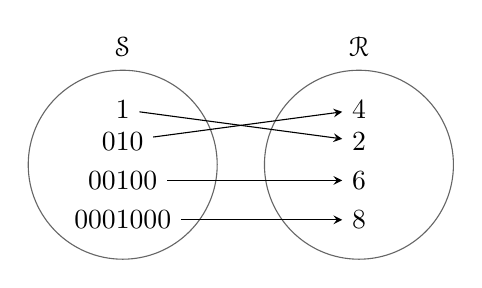
\begin{tikzpicture}
              % draw the sets
              \filldraw[fill=white!20, draw=black!60] (-1.5,0) circle (1.2cm);
              \filldraw[fill=white!20, draw=black!60] (1.5,0) circle (1.2cm);


              % the texts
              \node at (-1.5,1.5) {$\EuScript{S}$};
              \node at (1.5,1.5) {$\EuScript{R}$};

              % the points in the sets (here I just create nodes to use them later on to position
              % the circles and the arrows
              \node (x1) at (-1.5,0.7) {$1$};
              \node (x2) at (-1.5,0.3) {$010$};
              \node (x3) at (-1.5,-0.2) {$00100$};
              \node (x4) at (-1.5,-0.7) {$0001000$};
              \node (y1) at (1.5,0.7) {$4$};
              \node (y2) at (1.5,0.3) {$2$};
              \node (y3) at (1.5,-0.2) {$6$};
              \node (y4) at (1.5,-0.7) {$8$};

              % draw the arrows
              \draw[->] (x1) -- (y2);
              \draw[->] (x2) -- (y1);
              \draw[->] (x3) -- (y3);
              \draw[->] (x4) -- (y4);

          \end{tikzpicture}
        \end{center}
        From the mapping diagram, we conclude that $\Psi(\vb S) = \operatorname{len}(\vb S) + 1 $ is both injective
        and surjective, and hence its invertible.
          \end{proof}
      \end{solution}
    \item Come up with the correct formula for the inverse function $\Psi^{-1}$ and prove that your formula is
      correct using mapping tables. (\textbf{Hint:} The correct formula uses the floor function)
      \begin{solution}
        I claim that,
        \[
            \Psi^{-1} \colon \EuScript{R} \to \EuScript{S}\,,\,\,\, 
            \Psi^{-1}(r) = \operatorname{floor}\left( \frac{r - 1}{2}\right) \cdot \vb 0 + \vb 1 +
            \operatorname{floor}\left( \frac{r - 1}{2}\right) \cdot \vb 1
        .\] is the correct formula for the inverse function, where $\vb 0, \vb 1$ are binary bits. (They are being
        bolded just so we don't confuse them for integers $0,1$)

        \newpage

      \begin{proof}
        To prove our claim, it is sufficient to show that both conditions of Definition 4.1 hold using mapping
        tables,

          \begin{center}
            \begin{tabular}{c|c}
          \text{$\EuScript{S}$} & \text{$\Psi^{-1}\left( \Psi(\vb S) \right) $}\\\hline 
                $1$ & $\Psi^{-1}\left( \Psi(1) \right) = \Psi^{-1}\left( 2 \right)=
                \operatorname{floor}(0.5)\cdot \vb 0 + 1 + \operatorname{floor}(0.5) \cdot 0 = 0 \cdot \vb 0 + 1 +
                0 \cdot \vb 0 = 1$\\

                $010$ & $\Psi^{-1}\left( \Psi(010) \right) = \Psi^{-1}\left( 4 \right)=
                \operatorname{floor}(1.5)\cdot \vb 0 + 1 + \operatorname{floor}(1.5) \cdot 0 = 1 \cdot \vb 0 + 1 +
                1 \cdot \vb 0 = 010$\\

                $00100$ & $\Psi^{-1}\left( \Psi(00100) \right) = \Psi^{-1}\left( 6 \right)=
                \operatorname{floor}(2.5)\cdot \vb 0 + 1 + \operatorname{floor}(2.5) \cdot 0 = 2 \cdot \vb 0 + 1 +
                2 \cdot \vb 0 = 00100$\\

                $0001000$ & $\Psi^{-1}\left( \Psi(0001000) \right) = \Psi^{-1}\left( 8 \right)=
                \operatorname{floor}(3.5)\cdot \vb 0 + 1 + \operatorname{floor}(3.5) \cdot 0 = 3 \cdot \vb 0 + 1 +
                3 \cdot \vb 0 = 0001000$\\
          \end{tabular}

            \begin{tabular}{c|c}
          \text{$\EuScript{R}$} & \text{$\Psi\left( \Psi^{-1}(r) \right) $}\\\hline 
                $4$ & $\Psi\left( \Psi^{-1}(4) \right) = \Psi\left( 010 \right)= \operatorname{len}(010) + 1 = 3 +
                1 = 4$\\

                $2$ & $\Psi\left( \Psi^{-1}(2) \right) = \Psi\left( 1 \right)= \operatorname{len}(1) + 1 = 1 +
                1 = 2$\\

                $6$ & $\Psi\left( \Psi^{-1}(6) \right) = \Psi\left( 00100 \right)= \operatorname{len}(00100) + 1 
                = 5 + 1 = 6$\\

                $8$ & $\Psi\left( \Psi^{-1}(8) \right) = \Psi\left( 0001000 \right)= \operatorname{len}(0001000) + 1
                = 7 + 1 = 8$\\
          \end{tabular}
        \end{center}
        By our results from the mapping tables, we conclude that 
        \[
              \Psi^{-1}(r) = \operatorname{floor}\left( \frac{r - 1}{2}\right) \cdot \vb 0 + \vb 1 +
                  \operatorname{floor}\left( \frac{r - 1}{2}\right) \cdot \vb 1
        .\] is indeed the inverse function for $\Psi$.
        
        \end{proof}
        
      \end{solution}
  \end{enumerate}
\end{qstn}





























\end{document}




































